\section{Functional test procedure}
This chapter will help you to set up an infrastructure with one or several POP-C++ node and test it. 


\subsection{Test a single node}
The first thing to test is the single node installation. This test is done just to make sure that the Admin VM and the Worker VM are configured correctly to work together. \s

\textbf{Start the Global Services on the Admin VM}\\
First we need to start the POP-C++ Global Services on the Admin VM to be able to run a POP-C++ application. For this, use the following command:\s

\begin{lstlisting}
SXXpopc start
\end{lstlisting}\s

You should have a result as follows: \s

\begin{lstlisting}
Starting POP-C++ [Virtual Secure Version] Global Services
VSPSN Started [socket://160.98.21.238:54314] 
VPSM Started [socket://160.98.21.238:44603] 
POPCloner Started [socket://160.98.21.238:34485] 
VSJM Started [socket://160.98.21.238:2711] 
\end{lstlisting}\s

If you already have an error at this step, check the virtual configuration file located under \textit{POPC\_LOCATION} /etc/virtual.conf and be sure to have set the right parameters for your ESXi hypervisor and VMs.\s

Once the POP-C++ Global Service are started, we are ready to run a POP-C++ application on the node. For this, go to \textit{POPC\_RELEASE\_FOLDER}/demos/demopopc. We need to compile the code.\s

\begin{lstlisting}
make
\end{lstlisting}\s

Once the code is compiled, we need to provide a way to find this executable code. The easiest way is to put the code on a Web Server or FTP Server. The second way is to have a NFS. But for the second solution, we have to configure the Admin VM and Worker VM with the same NFS.\s

The most important is that the Worker VM can download the code to execute it. In our demo example, the code is \textbf{demopopc.obj}. This file must be accessible for the Worker VM. \s

Once the executable is accessible from somewhere, we need to edit the object map file. In our example, this file is named \textbf{obj.map}. Depending on the architecture, and location of the executable, this file could look like this. \s
\begin{lstlisting}
POPCobject i686-pc-Linux http://www.popcwebserver.com/example1/demoobj.obj
\end{lstlisting}


% #############################
% MULTIPLE NODES TEST
% #############################

\pagebreak
\subsection{Test several node}
To test the execution on several nodes, we first need to set up an infrastructure of POP-C++ nodes. We will set up 3 POP-C++ nodes to test two different aspects of POP-C++ VS.


%
% REFERENCE PASSING TEST
%
\subsubsection{Object reference passing test}

\textbf{Infrastructure schema}\\
Here is the connection schema of the infrastructure we would like to test. It's important to have two node that doesn't know each other. 
\begin{figure}[ht]
	\caption{Test Case 1: Logical Connection}
  	\centering
	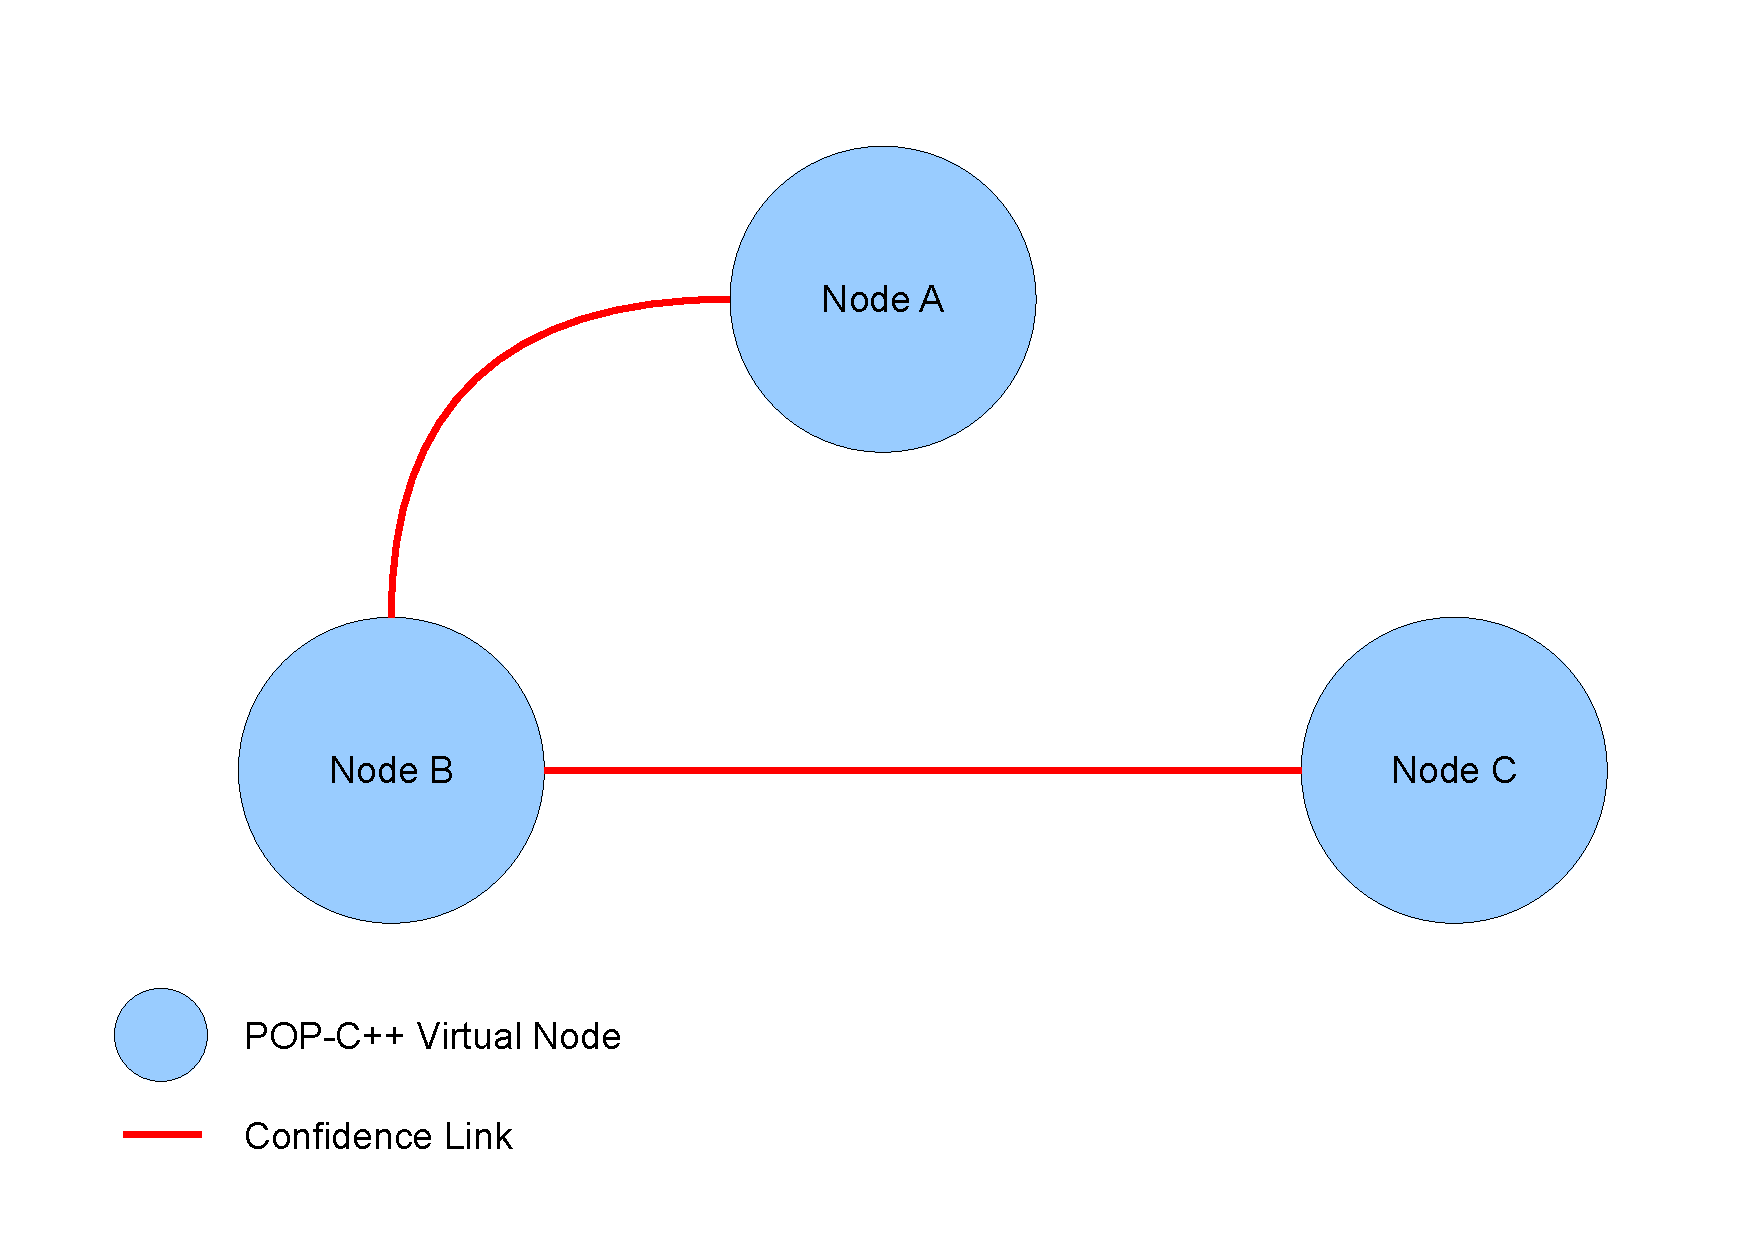
\includegraphics[width=0.7\textwidth]{./pic/testcase2.pdf}
	\label{fig:testcase1}
\end{figure}

\textbf{Infrastructure configuration}\\
\begin{itemize}
\item Node A has no master nodes. Node A has the PKI of Node B. The number of job is limited to 1 during the installation.
\item Node B has Node A as master node. Node B has the PKI of Node A and Node C. The number of job is limited to 1 during the installation.
\item Node C has Node B as master node. Node C has the PKi of Node B. The number of job is limited to 2 during the installation.
\end{itemize}
The Node A must be started first, Node B second and Node C after. \s


\textbf{Compilation and execution of test program}\\
To test this specific case, we will use the program located under \textit{POPC\_RELEASE\_FOLDER}/example/ multiobj/. To compile  this program, use the following command:\s

\begin{lstlisting}
make
\end{lstlisting}\s

As for the single node test, we need to provide a way to find the executable code. The file "demopopc.obj" must be uploaded on a Web or FTP server or located on a NFS drive. Once the file is accessible by and VM in the network, we must edit the obj.map file. Here is a sample of this file. \s
\begin{lstlisting}
POPCobject i686-pc-Linux http://www.popcwebserver.com/example1/demoobj.obj
\end{lstlisting}\s


Once the program is compiled and the executable accessible, use this command to run the program:\s
\begin{lstlisting}
popcrun obj.map ./main
\end{lstlisting}\s

Three Worker VM must be started on the three nodes. The program should end successfully. 


%
% DECENTRALIZED CREATION TEST
%

\subsubsection{Decentralized object creation test}
In this first test, we will check the creation of object by different nodes. \s

\textbf{Infrastructure schema}\\
Here is the connection schema of the infrastructure we would like to test. It's important to have one node between the first node (Main Node) and the last node. 
\begin{figure}[ht]
	\caption{Test Case 2: Logical Connection}
  	\centering
	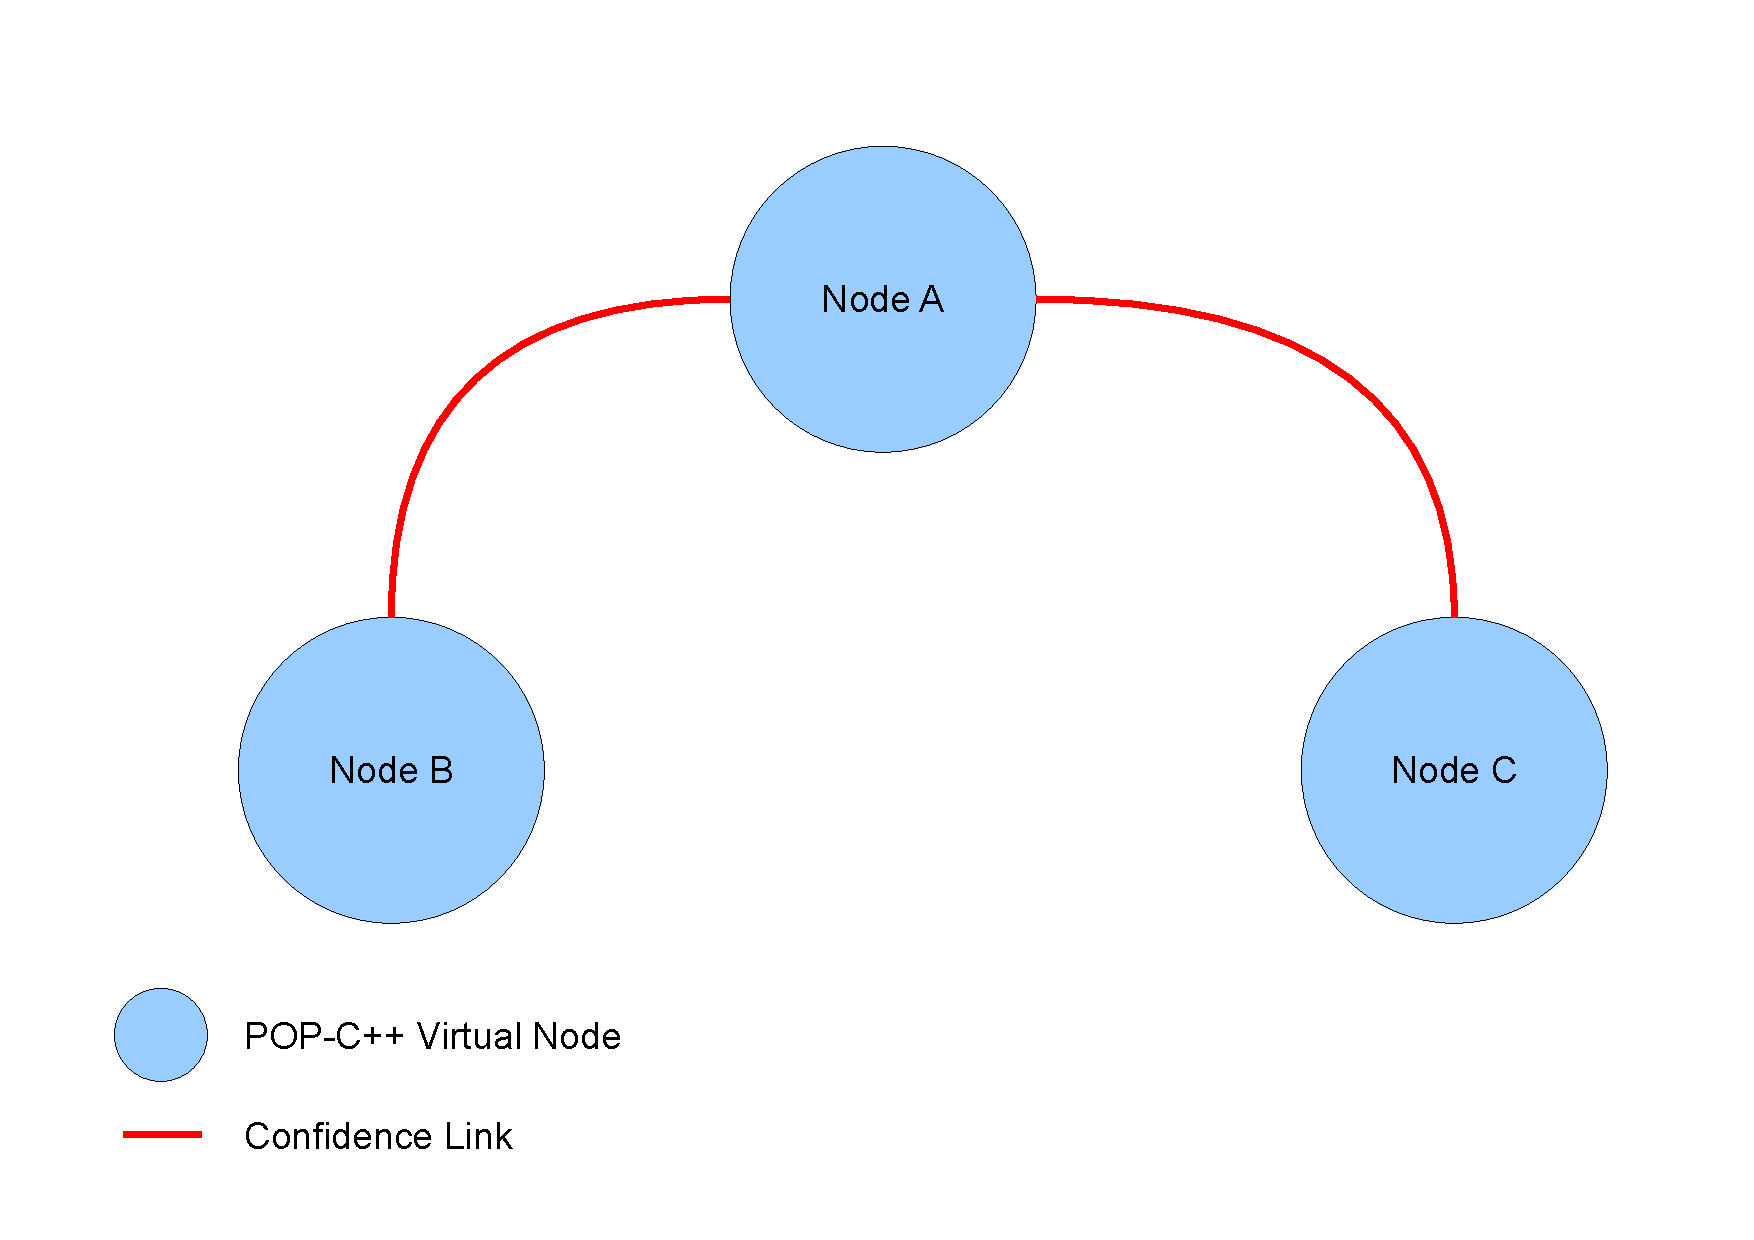
\includegraphics[width=0.7\textwidth]{./pic/testcase1.pdf}
	\label{fig:testcase1}
\end{figure}

\textbf{Infrastructure configuration}\\
\begin{itemize}
\item Node A has no master nodes. Node A has the PKI of Node B and Node C. The number of job is limited to 1 during the installation.
\item Node B has Node A as master node. Node B has the PKI of Node A. The number of job is limited to 1 during the installation.
\item Node C has Node A as master node. Node C has the PKi of Node A. The number of job is limited to 1 during the installation.
\end{itemize}
The Node A must be started first and Node B and C after. \s

\textbf{Compilation and execution of test program}\\
To test this specific case, we will use the program located under \textit{POPC\_REALEASE\_FOLDER}/demos/ demopopc/. To compile this program, use the following command:\s

\begin{lstlisting}
make
\end{lstlisting}\s

Once the program is compiled, use this command to run the program:\s
\begin{lstlisting}
popcrun objmap ./main 3 - - -
\end{lstlisting}\s

Three Worker VM must be started on the three nodes. The program should end successfully. 




\subsection{Test conclusion}
If the three tests have been executed successfully, we are now sure that our POP-C++ infrastructure is ready to execute our own program.





